\section{Discussion}

In this study, we made intrasubject comparisons of the accuracy (bias) and precision (inverse variance) characteristics in two spatial orientation tasks: SBT and SVV. The main experimental findings were as follows: (1) the SBT is more accurate than the SVV, (2) the SBT is less precise than the SVV, and (3) both SBT and SVV precision are smaller in tilted conditions than near upright. Under the assumption of optimality, a Bayesian model of sensory integration could account very well for these findings. Independent measurements, in supine subjects, of head-on-body variance confirmed the predicted value. 


\subsection{Comparison with previous work}
 
A world-vertical visual line appears tilted in space when the head is tilted in a darkened room (Aubert, 1861). Mittelstaedt (1983) was the first to emphasize that this phenomenon cannot be explained by errors in the body-tilt percept. He showed that subjects could accurately adjust themselves to a horizontal position, but, once in this position, made substantial systematic errors in the perception of visual verticality. Later, combined tests confirmed the discrepancy between SVV and SBT accuracy \cite{mast1996, jarchow1999, vanbeuzekom2000, vanbeuzekom2001, kaptein2004, vingerhoets2008}. The present study is consistent with these findings, showing substantial systematic SVV errors at tilts =60∞ and fairly accurate SBT performance. 

Compared with the abundant literature on SBT and SVV accuracy, data on their perceptual variability are scarce. In contrast to Mittelstaedt's observation (1983), Mast and Jarchow (1996) found that the SBT was much more variable than the SVV. The present study, the first to measure both SVV and SBT precision using an extensive psychometric approach, has clearly established that SBT variability is consistently higher than SVV variability, both in the upright and in the horizontal (90∞) tilt position. 

Furthermore, although various studies have noted that SVV variability increased at larger tilts \cite{schone1964, schone1968, udodehaes1970, vanbeuzekom2001, devrijer2008}, little is known about SBT variability as a function of tilt angle. Nelson (1968) showed that subjects were more variable when adjusting themselves to a horizontal position than to a vertical (upright) position. The present findings are consistent with these early observations. 


\subsection{Implications of the model}
 
After earlier indications that both the otoliths and body sensors contribute to the SBT (e.g., Clark and Graybiel, 1963, 1964; Nelson, 1968), Mittelstaedt (1997) made a quantitative assessment of their impact, using an ingeniously designed experiment. Subjects lay on their side in a horizontal centrifuge. The crux of the experiment was to vary the distance between the rotation axis and the interaural axis to equalize the opposite contributions from the otoliths and the body sensors so that the subject felt horizontal. By testing normal, paraplegic, and nephrectomized subjects, Mittelstaedt inferred how much each sensory system contributes to body-tilt perception. It was shown that, apart from the otoliths, also internal ``graviceptors'' in the trunk (such as the viscera) participate in the computation of the SBT. Later, some related studies provided evidence that the distribution of blood in the body also affects postural perception \cite{vaitl1997, vaitl2002}. According to Mittelstaedt (1998), the weight of the somatic graviceptors to estimate horizontal body orientation in healthy subjects is ~0.6 on average, with considerable intersubject variability. His estimate seems quite compatible with our wBD values at 90∞ tilt, which range between 0.35 (S5) and 0.93 (S6) (Fig. 5). 

Previous attempts to identify the separate contributions of the otoliths, neck, and body sensors on the SVV have yielded mixed results. Whereas Mittelstaedt (1998) found no evidence that the SVV was affected by the body sensors in his centrifuge experiment, other studies indicate that neck- and trunk-tilt aftereffects \cite{wade1968}, neck muscle vibration \cite{mckenna2004}, and manipulation of tactile and interoceptive body cues \cite{trousselard2004} can affect the SVV. In other words, even in the absence of direct head-in-space information from the otoliths, the brain can still obtain an estimate of head orientation in space through the indirect sensory pathway. These findings suggest that these modalities operate together with the otoliths in the computation of the SVV, consistent with our model. 


\subsection{Model evaluation}
 
The architecture of the model, as far as the reference frame transformations and the sensory integration is concerned, follows entirely from the principles of Bayesian inference. However, to account for our major findings and intersubject differences, we made two less straightforward assumptions. First, to explain the increased variability in both tasks at 90∞ tilt, we allowed for the possibility that the otoliths become more noisy with increases in tilt. Second, we hypothesized that prior knowledge is used in the visual vertical but not in body-tilt perception. Can these assumptions be justified on physiological and rational grounds? 

One reason to assume that otolith noise depends on tilt angle is based on the fact that the utricle contains considerably more hair cells than the saccule \cite{rosenhall1972, rosenhall1974}. Because the utricle is most sensitive to tilts of ~0∞, whereas the saccule is most sensitive at ~90∞ tilt \cite{jaeger2008}, this may well cause the proposed increase of otolith noise with tilt angle (Tarnutzer et al., 2010). A tilt-dependent noise level of the otoliths would also help to explain why the perturbing effect of roll-optokinetic stimulation on the SVV \cite{dichgans1974, fernandez1976} and on the SBT \cite{young1975} is more pronounced at larger tilt angles and why the SVV is more strongly influenced by residual canal signals at larger tilt angles, after prolonged roll rotations \cite{lorincz2008}.

In the SVV literature, it is widely assumed that the visual vertical is determined by a weighted combination of a sensory head-tilt signal and a head-fixed reference, denoted as the idiotropic vector \cite{mittelstaedt1983}. Recently, this idiotropic vector has been reinterpreted in terms of a Bayesian prior \cite{eggert1998, macneilage2007, devrijer2008}, with which it is mathematically equivalent. Interestingly, when tested in gravity-free conditions, subjects still retain a sense of visual vertical, always aligned with their long-body axis, compatible with the idea of head-fixed prior \cite{mittelstaedt1983}. Vingerhoets et al. (2008) recently found a similar phenomenon in the SVV during multiple-cycle dynamic roll rotation in normal gravity. Remarkably, when the same subjects were tested in a comparable dynamic SBT experiment, their responses showed very little bias on average, indicating that a prior is used only in the SVV and not for body-tilt estimation. To explain how this difference in computational approach might make sense, Vingerhoets et al. (2008) speculated that precision is more important than accuracy for the visual system, for reasons of visual stability. Combining the sensory tilt signal with prior knowledge yields a more stable percept of visual space than can be derived from the sensory signal alone. In a recent study, Bortolami et al. (2006) report virtually no bias in the haptically indicated vertical, which would be consistent with the suggestion that the prior plays primarily a role in visual processing. Likewise, for body-tilt perception, for which it might be less important to be precise and more useful to be accurate, the prior does not take part in this process. 

\subsection{Clinical implications}
 
According to our model, statistically optimal performance requires the use of information from both direct and indirect pathways to estimate body and head orientation in space (Fig. 1). Thus, if one of the sensory inputs is lost or severely disrupted, SBT and SVV performance will deteriorate, but should not completely break down due to their multimodality dependence. By setting the appropriate parameter values of the model to infinity, we simulated the model to predict SVV and SBT performance in two patient groups: bilateral vestibular patients (noise level of the otoliths set to infinity) and patients with somatosensory loss (noise level of the body sensors set to infinity). Figure 7 shows the results of these simulations. 

%\begin{figure}
\begin{wrapfigure}{l}[5pt]{0.5\textwidth}
    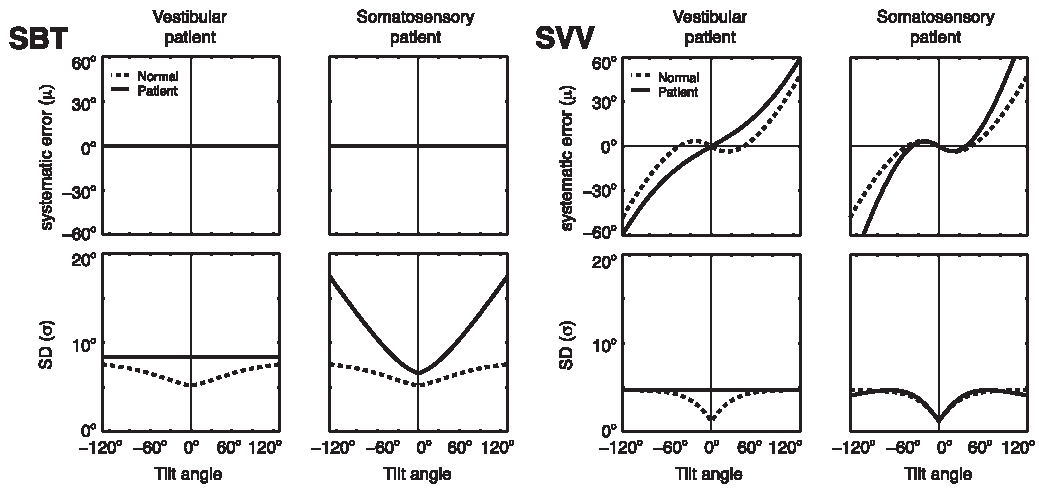
\includegraphics[width=0.5\textwidth]{src/paper1/figure7.pdf}
\end{wrapfigure}
%\end{figure}

When the otolith signal is lost (vestibular patient), the model predicts increased but constant noise levels in both the SBT and SVV, regardless of tilt angle. From the perspective of our model, the increased SBT variability can be attributed to the loss of the otolith contribution through the indirect body-in-space pathway. The increased bias in the SVV, predicted by the model, can also be understood: as the sensory-derived head-tilt estimate becomes noisier, the effect of the prior becomes more noticeable. Although there are no accuracy and variance measurements across the entire tilt range in these patients, the few previously published deficits are consistent with these predictions. Bisdorff et al. (1996) have shown that bilateral vestibular patients performed quite accurately in the SBT at upright, but were ~40\% more variable than normal subjects. Bronstein et al. (1996) showed that vestibular patients still compensated for their tilt angle when testing the SVV at 90∞, but with a bias about twice as large as in normal subjects, consistent with our simulations. 

The right column of Figure 7 depicts a simulation of the SBT and SVV in a patient with loss of somatosensory information (somatosensory patient). In this case, the SBT depends solely on otolith information mediated through the indirect pathway. Although this signal is still accurate, it is spoiled by the larger variability of the neck signal, needed to perform the appropriate reference frame transformation. The model also predicts larger errors in the SVV in these patients than in normal subjects. Although there are no reports containing measurements of bias and variance in the SBT and SVV, paraplegic patients show that along with the otoliths, internal body sensors also contribute to the SBT if lesions are below the 12th thoracic segment \cite{mittelstaedt1997}. This evidence supports the design of our model. 

In conclusion, we have tested the performance of healthy subjects in two psychophysical tasks that probe two spatial orientation estimates---SBT and SVV---and show that perceptual accuracy and precision in these tasks can be linked to the reference-frame-dependent weighting of sensory signals. We verified our theoretical framework by independent measurements of neck noise levels and by showing that it can account for the stereotypical performance of two patient groups. In this respect, our reverse-engineering approach also provides a new tool to establish diagnostic and prognostic markers of the quality of the signals involved in spatial orientation in neurological disease. 

\section{Appendix}

Here we provide further explanation about the Bayesian computations underlying the SVV as expressed in Equations 6 and 10 in Materials and Methods. Figure 8 illustrates graphically that the variance of the posterior distribution in a single trial (sH~S2) is not simply the same as the variance in its peak location in multiple trials, s2(H~S). In a single trial (Fig. 8A-C), the optimal estimate of head tilt is based on the likelihood (Fig. 8B, green curve) associated with the combined sensory input from the direct and the indirect pathway (Fig. 8A, green line, HS) and the prior (Fig. 8B, blue curve), by multiplication of the two probability distributions. The prior distribution is a Gaussian with mean HSP and variance sHSP2. The peak of the resulting posterior distribution (Fig. 8B, orange curve) is used as the optimal estimate of head tilt (H~S), given by the following: 

% Equation 13
\begin{equation}
\label{p1eqn13}
\tilde{H}_S = w_{HS} \cdot \hat{H}_S + w_{HP} \cdot H_{SP},
\end{equation}

with

% Equation 14
\begin{equation}
\label{p1eqn14}
w_{HS} = \frac{1 / \sigma^2_{HS}}{1 / \sigma^2_{HS} + 1 / \sigma^2_{HSP}},
\end{equation}

and

% Equation 15
\begin{equation}
\label{p1eqn15}
w_{HP} = \frac{1 / \sigma^2_{HSP}}{1 / \sigma^2_{HS} + 1 / \sigma^2_{HSP}},
\end{equation}

in which sHS denotes the noise in the sensory signal, known to the observer, and wHS and wHP represent the relative weights of the sensory signal and the prior, respectively. Note that Equation 13 is equivalent to Equation 1 in Materials and Methods. The variance of the posterior distribution in a single trial is given by the following: 

% Equation 16
\begin{equation}
\label{p1eqn16}
\sigma^2_{HS} = w_{HS} \cdot \sigma^2_{HS} \\
              = \frac{\sigma^2_{HSP}}{\sigma^2_{HS} + \sigma^2_{HSP}} \cdot \sigma^2_{HS}
\end{equation}

and is reflected by the width of the orange curve in Figure 8B. Figure 8D-F illustrates performance in multiple trials, in which the posterior distributions vary due to sensory noise (sHS), whereas the prior remains fixed. The variance of each posterior distribution is fixed and is given by Equation 16. 

%\begin{figure}
\begin{wrapfigure}{l}[5pt]{0.75\textwidth}
    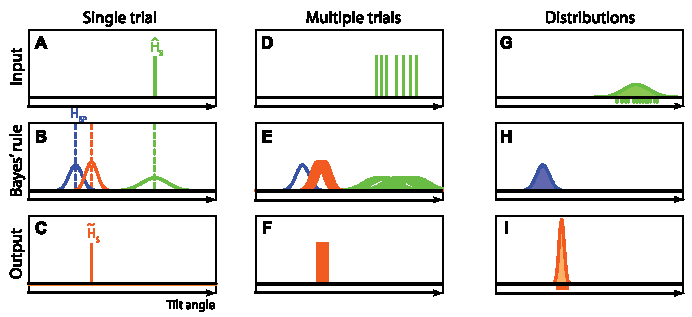
\includegraphics[width=0.75\textwidth]{src/paper1/figure8.pdf}
%\end{figure}
\end{wrapfigure}

That the variance of the peak locations across multiple trials, $\sigma^2(\tilde{H}_S)$, is smaller can be shown by applying the rules of noise propagation to Equation 13. 

% Equation 17
\begin{equation}
\label{p1eqn17}
\sigma^2(\tilde{H}_S) = \\
	\big( \frac{\delta\tilde{H}_S}{\delta\hat{H}_S^2} \big) \cdot \\
	\sigma^2(\hat{H}_S) + \\
	\big( \frac{\delta\tilde{H}_S}{\delta H_{SP}^2} \big) \cdot \\
	\sigma^2(H_{SP}) \\
	= w^2_{HS} \cdot \sigma^2_{HS} \\
	= \frac{\sigma^2_{HSP}}{\sigma^2_{HS} + \sigma^2_{HSP}} \cdot \sigma^2_{HS}
\end{equation}

which is equivalent to Equation 10 in Materials and Methods. Corresponding panels G-I (Fig. 8) illustrate the distribution of the sensory signals for a given tilt angle (green-shaded curve), the prior distribution (blue-shaded curve), and the optimal estimates (orange-shaded curve), respectively. Figure 8I illustrates that the distribution of the optimal estimates across many trials has a lower variance than the posterior distribution in each single trial (Fig. 8B), which follows from the comparison of Equations 16 and 17, respectively. 
